\chapter{Integration I}

In this chapter we will present an introduce integration over oriented intervals and generalise to higher dimensions.
For the time being, we will focus on the intuition behind this and only worry about axis-aligned $n$-cubes.
Following this, in the next chapter, we will delve more deeply from a measure theoretic perspective and integration over more general shapes.

%%%%%%%%%%%%%%%%%%%%%%%%%%%%%%%%%%%%%%%%%
%
% SINGLE VARIABLE
%
%%%%%%%%%%%%%%%%%%%%%%%%%%%%%%%%%%%%%%%%%

\section{Single variable integration}

Given a function $f$ with real variable $x$ and an interval $[a,b)$ on the (extended) real line, 
a traditional \textbf{definite integral} would be of the form:
\begin{equation*}
	\int_a^b f(x) \; dx \;\;\;\;\; \text{or} \;\;\;\;\; \int_{[a,b)} f(x) \; dx
\end{equation*}
Which we interpret as the signed area bounded by $f$ between $x=a$ and $x=b$.
However, defining this definite integral using (unoriented) intervals like this is a bit of a misnomer.
In the case where $a \geq b$ one would typically use the identity:
\begin{equation}
	\int_a^b f(x) \; dx = - \int_b^a f(x) \; dx
\end{equation}
to evaluate the integral.
But, as we saw in the previous chapter, when $a \geq b$, the interval $[a,b)$ is the empty set!
We can't translate equation (4.1) to an identity along the lines of:
\begin{equation}
	\int_{[a,b)} f(x) \; dx = - \int_{[b,a)} f(x) \; dx
\end{equation}
since at least one of $[a,b)$ or $[b,a)$ will be always be empty.
Although this notation generally appears in context of Lebesgue integrals, 
Riemann integrals (which generally use $\int_a^b ...$ instead) simply hide this mis-use of intervals.
For example, 
\todo[inline]{Find one that's not wikipedia!

- tagged partition given as a series $x_i$ such that $a = x_1 < x_2 < ... < x_n = b$ which we say is the integral $\int_a^b$

- Unintentionally we are claiming that $\int_1^0 f(x) \; dx = \int_{[1,0]}= \int_{\emptyset} f(x) \; dx = 0$
}

If oriented intervals are used instead of traditional intervals, then the identity from equation (4.1) can instead just be a result of \emph{bi-linearity}.
\begin{equation}
	\int_{[\![a,b)\!)} f(x) \; dx = - \int_{\ominus [\![a,b)\!)} f(x) \; dx = - \int_{[\![b,a)\!)} f(x) \; dx
\end{equation}


\begin{definition}
	Let $[\![ a,b ]\!]$ be an interval on $\mathbb{R}$ then the boundary function $\partial$ is the linear map such that:
	\begin{equation}
		\partial( \;[\![a,b]\!]\; ) = \hset{ a^1, b^{-1} }
	\end{equation}
\end{definition}

\todo[inline]{ By linearity we also have:

$\partial (\!(a,b)\!) = \partial ( \; \ominus [\![b,a]\!] \; )= \ominus \partial ( \; [\![b,a]\!] \; ) = \ominus \hset{ b^1, a^{-1} } = \hset{ a^1, b^{-1}}$.

Using this we also have:}

$\partial [\![a,b)\!) = \partial ( [\![a,c]\!] \oplus (\!(c,b)\!) ) = \partial [\![a,c]\!] \oplus \partial (\!(c,b)\!) =  \hset{ a^1, c^{-1} } \oplus \hset{ c^1, b^{-1} } = \hset{a^1, b^{-1} }$


And by a similar proof for $\partial (\!(a,c]\!]$, we conclude that:
\begin{equation}
	\partial [\![a,b]\!] = \partial [\![a,b)\!) = \partial (\!(a,b]\!] = \partial (\!(a,b)\!)
\end{equation}


Isolated points do not affect the boundary of an oriented interval.
This should have been obvious from the definition to begin with.
The interval $[\![ a,a ]\!]$ is a hybrid set which contains only the element $a$ with multiplicity one.
From equation XX,
\begin{equation}
	\partial [\![ a,a ]\!] = \hset{a^1, a^{-1}} = \emptyset
\end{equation}

So whether we use $\int_a^b$ to denote the integral over the intervals $[\![a,b]\!]$, $[\![a,b)\!)$ or  $(\!(a,b)\!)$ the boundary is unchanged and so the integral will evaluate identically.

The hybrid sets $[\![a,b]\!] \oplus [\![b,c]\!]$ and $(\!(a,b)\!) \oplus (\!(b,c)\!)$ have identical multiplicities almost everywhere.
At $b$, they will differ by 2. 
Although simple arguments resolve this issue, by using left-closed, right-open oriented intervals we can bypass these arguments altogether when showing
\begin{equation}
	\int_{[\![a,b)\!)} f(x) \; dx + \int_{[\![b,c)\!)} f(x) \; dx = \int_{[\![a,c)\!)} f(x) \; dx
\end{equation}

%%%%%%%%%%%%%%%%%%%%%%%%%%%%%%%%%%%%%%%%%
%
% N-CUBES
%
%%%%%%%%%%%%%%%%%%%%%%%%%%%%%%%%%%%%%%%%%

\section{Higher dimension intervals}

For now, we will concern ourselves only with oriented, $n$-dimensional, axis-aligned rectangles in $\mathbb{R}^n$.
In one dimension, the previously discussed oriented intervals cover most of the ``obvious shapes'' one would be interested in.
Moving to two dimensions, there are many more ``obvious shapes'' to consider but we will temporarily ignore triangles, circles and even rectangles that are tilted.
We could also use triangles instead of rectangles as our primitive of choice. 
This would generalize to $n$-simplexes in higher dimensions.
Since $n$-simplexes and $n$-cubes end up b\cite{choquetanalysis}
But, first we must introduce some notation to describe these and higher dimension rectangles. 

At the moment the only rectangles we have defined are the one-dimensional ``oriented interval''.
Hence we will also refer to this as a 1-cube.
We construct higher dimensional $n$ rectangles using the Cartesian product.
\begin{definition}
	Let $X = \hset{ x_1^{m_1}, ... , x_k^{m_k} }$ and $Y= \hset{ y_1^{n_1}, ... , y_\ell^{n_\ell} }$ be hybrid sets.
	We define the \textbf{Cartesian product of hybrid sets $\boldsymbol{X}$ and $\boldsymbol{Y}$}, denoted with $\times$ operator as:
	\begin{equation}
		X \times Y = \hset{ (x, y)^{m \cdot n} \; : \; x^m \in X, y^n \in Y }
	 \end{equation}
\end{definition}

If $[\![a,b]\!]$ and $[\![c,d]\!]$ are both positively oriented 1-rectangles then their Cartesian product is shown in Figure 4.1 is clearly a two dimensional rectangle or \emph{2-rectangle}. 
Taking the Cartesian product of a 2-rectangle and 1-rectangle gives a 3-rectangle in $\mathbb{R}^3$. 
We should note here that we do not distinguish between $((x,y),z)$ and $(x,(y,z))$ but rather we treat both as different names for the ordered triple $(x,y,z)$.
We similarly associate parentheses in higher dimensions as well.

\begin{figure}[h]
\caption[Cartesian product of two 1-rectangles]{The Cartesian product of two positively oriented 1-rectangles $[\![a,b]\!]$ and $[\![c,d]\!]$ is a positively oriented 2-rectangle.}
\centering
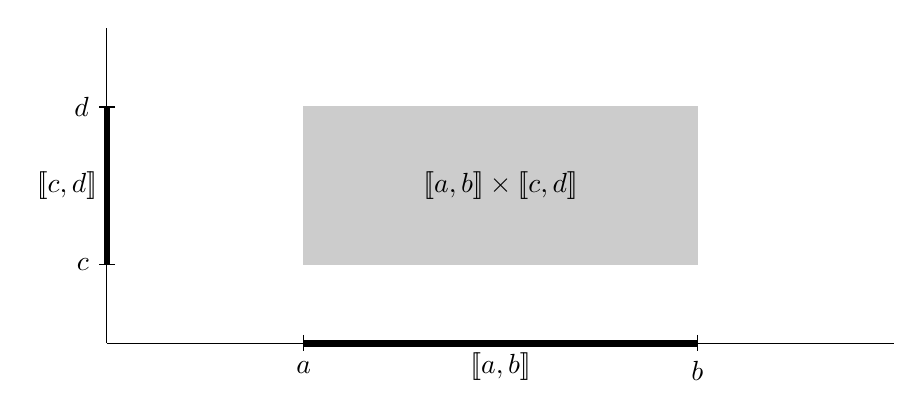
\begin{tikzpicture}[y=1cm, x=2.5cm]	
 	%axis
	\draw(0,0) -- coordinate (x axis mid) (4,0);
    	\draw (0,0) -- coordinate (y axis mid) (0,4);
    	
    	%ticks
    	\draw[fill] (1,1pt) rectangle (3,-1pt);    	
    	\draw (1, 3pt) -- (1, -3pt) node[anchor=north] {$a$};
    	\draw (3, 3pt) -- (3, -3pt) node[anchor=north] {$b$};
    	\draw (2, 0) node[anchor=north] {$[\![a,b]\!]$};
    	
    	\draw[fill] (1pt,1) rectangle (-1pt, 3);
    	\draw (3pt, 1) -- (-3pt, 1) node[anchor=east] {$c$};
    	\draw (3pt, 3) -- (-3pt, 3) node[anchor=east] {$d$};
    	\draw (0,2) node[anchor=east] {$[\![c,d]\!]$};
    	
    	\draw[fill, color=black!20] (1,1) rectangle (3,3);
    	\draw (2, 2) node {$[\![a,b]\!] \times [\![c,d]\!]$ };
\end{tikzpicture}
\end{figure}

\begin{theorem}
	The Cartesian product of a $k$-rectangle in $\mathbb{R}^m$ (where, $k\leq m$) 
	and $\ell$-rectangle in $\mathbb{R}^n$ (again, $\ell \leq n$) 
	is a $(k+\ell)$-rectangle in $\mathbb{R}^{m+n}$.
\end{theorem}

For completeness we will also define a 0-rectangle as a hybrid set containing a single point with multiplicity $1$ or $-1$.
Firstly this allows us to embed $k$-rectangles in $\mathbb{R}^n$.
For example $[\![a,b]\!] \times [\![c,d]\!] \times \hset{e^1}$ is the product of two 1-rectangles and a 0-rectangle (all over $\mathbb{R}$) and so it is a 2-rectangle over $\mathbb{R}^3$.
Specifically, it is the 2-rectangle $[\![a,b]\!] \times [\![c,d]\!]$ on the plane $z=3$.
This also illustrates the principle that given a $k$-rectangle in $\mathbb{R}^n$ where $n>k$ we can always find a $k$ dimensional subspace which also contains the rectangle.
We will re-use the interval notation from earlier although one should be careful to ``type-check'' while interpreting.
When $a$ and $b$ are real numbers then we continue to use the definition $[\![a,b]\!] = [a,b) \ominus [b,a)$.
However, when $\boldsymbol{a}$ and $\boldsymbol{b}$ are $n$-tuples (for example, coordinates in $\mathbb{R}^n$ then this is \emph{not} the oriented line interval $[\boldsymbol{a}, \boldsymbol{b}) \ominus [\boldsymbol{b}, \boldsymbol{a})$.

\begin{definition}
	Let $\boldsymbol{a} = (a_1, a_2, \ldots, a_n)$ and 
	$\boldsymbol{b} = (b_1, b_2, \ldots, b_n)$ be ordered $n$-tuples then we use the notation:
	\begin{align}
		[\![ \boldsymbol{a}, \boldsymbol{b} ]\!] 
		= [\![a_1, b_1]\!] \times [\![a_2, b_2 ]\!] \times \ldots \times [\![a_n , b_n]\!]
	\end{align}
\end{definition}

The dimension of $[\![ \boldsymbol{a}, \boldsymbol{b} ]\!]$ is equal to the number of indices where $a_i$ and $b_i$ are distinct.
For any $i$ where $a_i = b_i$, the corresponding term: $[\![ a_i, b_i ]\!]$ will be a hybrid set containing a single point, that is, a 0-rectangle.
The orientation of $[\![ \boldsymbol{a}, \boldsymbol{b} ]\!]$ is based on the number of negatively oriented intervals $[\![a_i,b_i]\!]$.
Should there be an odd number of indices $i$ such that $a_i > b_i$ then $[\![ \boldsymbol{a}, \boldsymbol{b} ]\!]$ will also be negatively oriented.
Otherwise, it will be positively oriented. 

%%%%%%%%%%%%%%%%%%%%%%%%%%%%%%%%%%%%%%%%%
%
% RIEMANN
%
%%%%%%%%%%%%%%%%%%%%%%%%%%%%%%%%%%%%%%%%%

\section{Riemann Integral on $n$-cubes}

Now that we have oriented $n$-dimensional cubes, we would like to define the integral over one.
For now, we will content ourselves with the Riemann integral and Euclidean volume.
More complex domains and other metrics will be handled in later chapters with push-backs and the Lebesgue integral.
The volume of an oriented $n$-cube in $\mathbb{R}^n$ we define to be the product of its side lengths.
Formally,

\begin{definition}
	Let $[\![\boldsymbol{a}, \boldsymbol{b}]\!]$ be a $k$-cube in $\mathbb{R}^n$ again with $\boldsymbol{a}=(a_1,\ldots, a_n)$ and $\boldsymbol{b}=(b_1,\ldots, b_n)$. 
	We denote the \textbf{volume of $\boldsymbol{[\![a,b]\!]}$} with $\text{vol}$ and define it as:
	\begin{equation}
		\text{vol}(\; [\![\boldsymbol{a}, \boldsymbol{b} ]\!] \;) = (b_1 - a_1) \cdot (b_2 - a_2) \cdot \ldots \cdot (b_n - a_n)
	\end{equation}
\end{definition}

For any $k<n$, a $k$-cube will have volume zero.
In at least one dimension, the cube will be degenerate (i.e. $a_i = b_i$) and so will contribute zero to the product.
Additionally, one can also observe that $\text{vol}( \ominus [\![\boldsymbol{a}, \boldsymbol{b} ]\!]) = - \text{vol}( [\![ \boldsymbol{a}, \boldsymbol{b} ]\!]$.


\todo{image instead of tikz?}
\begin{figure}[h]
\caption[Riemann Integral]{Riemann Integral visual example.}
\centering
\begin{tikzpicture}[scale=2, domain=0:5]
	\draw[<->] (0,2) -- (0,0) -- (5,0);
	\draw[smooth,samples=20, domain=0.0:5.0] plot(\x, {(\x^3 - 6 * \x^2 + 4 * \x + 18)/10});
\end{tikzpicture}
\end{figure}

Given an $n$-cube $[\![\boldsymbol{a}, \boldsymbol{b}]\!]$ we must cut each $[\![a_i, b_i]\!]$ into partitions.
Previously we used generalized partitions and did not mind if pieces overlapped or exceeded the original range.
However, for building our Riemann sums, we are only interested in partitions in the traditional, non-intersecting sense.

\begin{definition}
	Given an oriented interval $[\![a,b]\!]$ of the real line, we say that a partition of $[\![a,b]\!]$, $\{P_i\}_{i=1}^n$
	is an \textbf{interval partition of $\boldsymbol{[\![a,b]\!]}$} if its pieces are:
	\begin{enumerate}
		\item \emph{Oriented intervals}: $P_i$ is an oriented interval of the real line for all $i$.
		\item \emph{Disjoint}: $P_i \otimes P_j = \emptyset$ for all $i,j$
	\end{enumerate}
	We denote the set of all such partition as $\mathcal{P}[\![a,b]\!]$.
\end{definition}

This greatly restricts the types of partitions we have access to.
Every interval partition will be --- up to substitution of ``$]\!], (\!($'' in place of ``$)\!), [\![$'' --- of the form:
\begin{equation}
	\Big\{ \; [\![a,x_1)\!), \; [\![x_1, x_2)\!), \; [\![x_2, x_3)\!),\; \ldots,\; [\![x_{n-1}, b]\!] \; \Big\}
\end{equation}
where $x_i$ is a monotone sequence (that is, either non-increasing or non-decreasing).
This is not to say that $P_i = [\![x_{i-1}, x_i )\!)$ as the pieces of $P$ may not be given in this order.
Regardless of the ordering, we select partitions $P^j \in \mathcal{P}[\![a^j,b^j)\!)$ for each dimension of $[\![a,b)\!)$.
To build our mesh, we construct smaller $n$-cubes $I_{i_1, \ldots, i_n}$ using the Cartesian product of pieces:
\begin{equation}
	I_{i_1, \ldots, i_n} = i_1 \times \ldots \times i_n
\end{equation}
where each $i_j$ is taken from $P^j$.
We are now ready to construct Riemann sums.

\begin{definition}
	Given $P=\{ P_j \}_{j=1}^n$ where $P_j \in \mathcal{P}[\![a_j, b_j]\!]$,
	and $f:[\![\boldsymbol{a}, \boldsymbol{b}]\!] \to \mathcal{R}$ then we define a Riemann sum $f_P$ to be:
	\begin{equation}
		f_P = \sum_{i_1 \in P_1} \ldots \sum_{i_n \in P_n} f(x_{i_1, \ldots, i_n}) \text{vol}(I_{i_1, \ldots, i_n})
	\end{equation}
	where $x_{i_1, \ldots, i_n}$ is any point chosen from $I_{i_1, \ldots, i_n}$.
\end{definition}

\todo[inline]{``a'' not ``the''. left, right, trapezoidal,upper, lower,...}

Recall our discussion of refinements from Chapter 2.
Given 2 partitions $P$ and $P'$ of the same set then we say $P \preceq P'$ if $P'$ is a refinement of $P$.
In this way we can induce a partial ordering on $\mathcal{P}[\![a,b]\!]$.
There is a unique smallest element in this partial ordering which is $[\![a,b]\!]$ itself; 
every partition by definition will refine $[\![a,b]\!]$.

\todo[inline]{Given $P$ and $P'$ can always find $Q$ such that $P \preceq Q$ and $P' \preceq Q$}

As we go up in our ordering, our mesh becomes increasingly fine.
Taking the Riemann sum of the suprema of this poset gives us the Riemann integral.

\begin{definition}
The Riemann integral of a function $f:\mathbb{R}^n \to \mathbb{R}$ over a $k$-cube $[\![\boldsymbol{a}, \boldsymbol{b}]\!]$
where P is $\sup \{ \mathcal{P} [\![a,b]\!] \}$
	\begin{equation}
		\int_{[\![a,b]\!]} f(x) \; dx = f_{\sup \{ \mathcal{P} [\![a,b]\!] \}}
	\end{equation} 
\end{definition}

\todo[inline]{Riemann integrable. upper and lower approach}

%%%%%%%%%%%%%%%%%%%%%%%%%%%%%%%%%%%%%%%%%
%
% BOUNDARY
%
%%%%%%%%%%%%%%%%%%%%%%%%%%%%%%%%%%%%%%%%%

\section{Boundary Operator}

In one dimension, the boundary of an interval was quite straight-forward.
For a positively oriented interval, the boundary was composed of two points; 
the right end-point was positive and the left end-point was negative.
From the perspective of $k$-rectangles, 
the $\partial$ operator has mapped an oriented 1-rectangle to a set of oriented 0-rectangles.
We will now generalize the boundary to map an oriented $n$-rectangle to an $(n-1)$-rectangle.

\begin{definition}
	Let  $[\![\boldsymbol{a}, \boldsymbol{b}]\!]$ be a a $k$-rectangle in $\mathbb{R}^n$.
	Additionally, let $i_1, i_2, \ldots, i_k$ be the unique non-decreasing sequence of indices such that $a_{i_j} \neq b_{i_j}$.
	The \textbf{boundary of $ \boldsymbol{[\![ a,b ]\!]} $ }, denoted the operator $\partial$ is given by
	\begin{align}
		\partial \left( [\![ \boldsymbol{a}, \boldsymbol{b} ]\!] \right) 
		= \bigoplus_{j=1}^k (-1)^j \;
			\left(	
			[\![ \boldsymbol{a}^{[\![1,i_j)\!)}, \boldsymbol{b}^{[\![1,i_j)\!)} ]\!]
			\times \hset{a_{i_j}} \times \right. &
			[\![ \boldsymbol{a}^{(\!(i_j,n]\!]}, \boldsymbol{b}^{(\!(i_j,n]\!]} ]\!]  \notag\\
			\ominus
			[\![ \boldsymbol{a}^{[\![1,i_j)\!)}, \boldsymbol{b}^{[\![1,i_j)\!)} ]\!]
			\times \hset{b_{i_j}} \times & \left.
			[\![ \boldsymbol{a}^{(\!(i_j,n]\!]}, \boldsymbol{b}^{(\!(i_j,n]\!]} ]\!]
			\right)
	\end{align}
\end{definition}

The above equation will require a bit of unpacking to digest featuring oriented intervals in two different contexts.
The first appears in the superscripts of $\boldsymbol{a}$ and $\boldsymbol{b}$. 
The intervals $[\![1, i_j)\!)$ and $(\!(i_j, n]\!]$ are  and is an interval over vector indices just as in Chapter 3.
Thus, the term $\boldsymbol{a}^{[\![1,i_j)\!)}$ refers to the vector $(a_1, a_2, \ldots, a_{i-1})$ 
while the term $\boldsymbol{b}^{(\!(i,n]\!]}$ refers to $(b_{i+1}, b_{i+2}, \ldots, b_{n})$.
This provides a compact notation to partition the original range of indices into 3 pieces: $[\![ 1,i )\!)$, $[\![i, i]\!]$, and $(\!(i, n]\!]$.
The first and last portions are isolated but left untouched, 
but the central $[\![i,i]\!]$ term is then replaced with the 0-rectangles $a_i$ or $b_i$.
Formally, we are actually using the hybrid sets $\hset{(a_i)^1}$ and $\hset{(b_i)^1}$ but we omit the explicit multiplicity of one (and will continue to do so through out the section) to lighten notation.

Each Cartesian product forms a $(k-1)$-rectangular face of the $k$-rectangle which we shall show.
Let $[\![ \boldsymbol{a}, \boldsymbol{b} ]\!]$ be a $k$ rectangle in $\mathbb{R}^n$.
Following from definitions we have:
\begin{equation}
	[\![ \boldsymbol{a}, \boldsymbol{b} ]\!] = 
		[\![\boldsymbol{a}^{[\![1,i)\!)}, \boldsymbol{b}^{[\![1,i)\!)} ]\!] \times 
		[\![\boldsymbol{a}^{[\![i,i]\!]}, \boldsymbol{b}^{[\![i,i]\!]} ]\!] \times
		[\![\boldsymbol{a}^{(\!(i,n]\!]}, \boldsymbol{b}^{(\!(i,n]\!]} ]\!]
\end{equation}
If $a_i$ and $b_i$ are distinct then $[\![\boldsymbol{a}^{[\![i,i]\!]}, \boldsymbol{b}^{[\![i,i]\!]} ]\!]$ is a 1-rectangle.
Since both $a_i$ and $b_i$ are 0-rectangles and expressions agree everywhere else, then the following are both $(k-1)$-rectangles:
\begin{align}
	[\![\boldsymbol{a}^{[\![1,i)\!)}, \boldsymbol{b}^{[\![1,i)\!)} ]\!]
	\times \hset{a_i} \times
	[\![\boldsymbol{a}^{(\!(i,n]\!]}, \boldsymbol{b}^{(\!(i,n]\!]} ]\!]
	\\
	[\![\boldsymbol{a}^{[\![1,i)\!)}, \boldsymbol{b}^{[\![1,i)\!)} ]\!]
	\times \hset{b_i} \times
	[\![\boldsymbol{a}^{(\!(i,n]\!]}, \boldsymbol{b}^{(\!(i,n]\!]} ]\!]
\end{align}
However if $a_i = b_i$ then $[\![\boldsymbol{a}^{[\![i,i]\!]}, \boldsymbol{b}^{[\![i,i]\!]} ]\!]$ is a 0-rectangle and so the expressions in (4.10) and (4.11) are both $k$-rectangles!
Since $a_i = b_i$, the two expressions are identical, so their difference is zero and the terms disappear.

\subsection{Example: \emph{Boundary of a 1-rectangle}}

Let $\boldsymbol{a}= (a_1)$ and $\boldsymbol{b} = (b_1)$ be trivial 1-tuples. 
It follows that:
\begin{align*}
	\partial ( \; [\![ \boldsymbol{a}, \boldsymbol{b} ]\!] \; )
	=& \; (-1)^i ( [\![\boldsymbol{a}^{[\![1,1)\!)}, \boldsymbol{b}^{[\![1,1)\!)} ]\!]
	\times \hset{a_1} \times
	[\![\boldsymbol{a}^{(\!(1,1]\!]}, \boldsymbol{b}^{(\!(1,1]\!]} ]\!]\\
	&\; \ominus
	[\![\boldsymbol{a}^{[\![1,1)\!)}, \boldsymbol{b}^{[\![1,1)\!)} ]\!]
	\times \hset{b_1} \times
	[\![\boldsymbol{a}^{(\!(1,1]\!]}, \boldsymbol{b}^{(\!(1,1]\!]} ]\!] )\\
	=& \; \ominus [\![\boldsymbol{a}^{\emptyset}, \boldsymbol{b}^{\emptyset} ]\!]
	\times \hset{a_1} \times
	[\![\boldsymbol{a}^{\emptyset}, \boldsymbol{b}^{\emptyset} ]\!]\\
	& \; \oplus
	[\![\boldsymbol{a}^{\emptyset}, \boldsymbol{b}^{\emptyset} ]\!]
	\times \hset{b_1} \times
	[\![\boldsymbol{a}^{\emptyset}, \boldsymbol{b}^{\emptyset} ]\!] \\
	=& \; \hset{b_1} \ominus \hset{a_1}
\end{align*}
Again, we omit the braces from the hybrid sets $\hset{(a_1)^1}$ and $\hset{(b_1)^1}$.
Recalling from the previous section in equation (4.4), we can see that the results agree:
\begin{equation}
	\partial ( \; [\![ a_1 ,b_1 ]\!] \; ) = \hset{b_1} \ominus \hset{a_1} = \hset{(b_1)^1} \ominus \hset{(a_1)^1} = \hset{(a_1)^{-1}, (b_1)^1}
\end{equation}

\subsection{Example: \emph{Boundary of a 3-rectangle}}
Let $\boldsymbol{a} = (0,0,0)$ and $\boldsymbol{b} = (1,1,1)$.
Omitting the intermediate step, we find the boundary of $[\![ \boldsymbol{a}, \boldsymbol{b} ]\!]$ to be:
\begin{align*}
	\partial ( \; [\![ \boldsymbol{a} , \boldsymbol{b} ]\!] \; ) =
	& 	\; \ominus \; \left( \hset{0} \times [\![0,1]\!] \times [\![0,1]\!] \right)
		\; \oplus \; \left( \hset{1} \times [\![0,1]\!] \times [\![0,1]\!] \right)
	\\& 	\; \oplus \; \left( [\![0,1]\!] \times \hset{0} \times [\![0,1]\!] \right)
	 	\; \ominus \; \left( [\![0,1]\!] \times \hset{1} \times [\![0,1]\!] \right)
	\\& 	\; \ominus \; \left( [\![0,1]\!] \times [\![0,1]\!] \times \hset{0} \right)
	  	\; \oplus \; \left( [\![0,1]\!] \times [\![0,1]\!] \times \hset{1} \right)
\end{align*}

This may not be the most enlightening expression on its own.
In Figure 4.3 below, the 3-rectangle given by $[\![\boldsymbol{a}, \boldsymbol{b}]\!]$ can be seen as a cube in three dimensions.
Physically, the 3-rectangle is a solid cube and includes all interior points.
The boundary meanwhile are just the rectangular outer faces, which conveniently,
 there are also six to match the six terms of $\partial[\![\boldsymbol{a},\boldsymbol{b}]\!]$.

\begin{figure}[h]
\caption[Unit cube with boundary]{The unit cube in $\mathbb{R}^3$ with positive orientation can be represented as the 3-rectangle: $[\![(0,0,0), (1,1,1) ]\!]$ is shown as a wire-frame. 
The six faces that make up its boundary are shaded and labeled with their corresponding terms.
%Now with 100% more right-handed
}
\centering
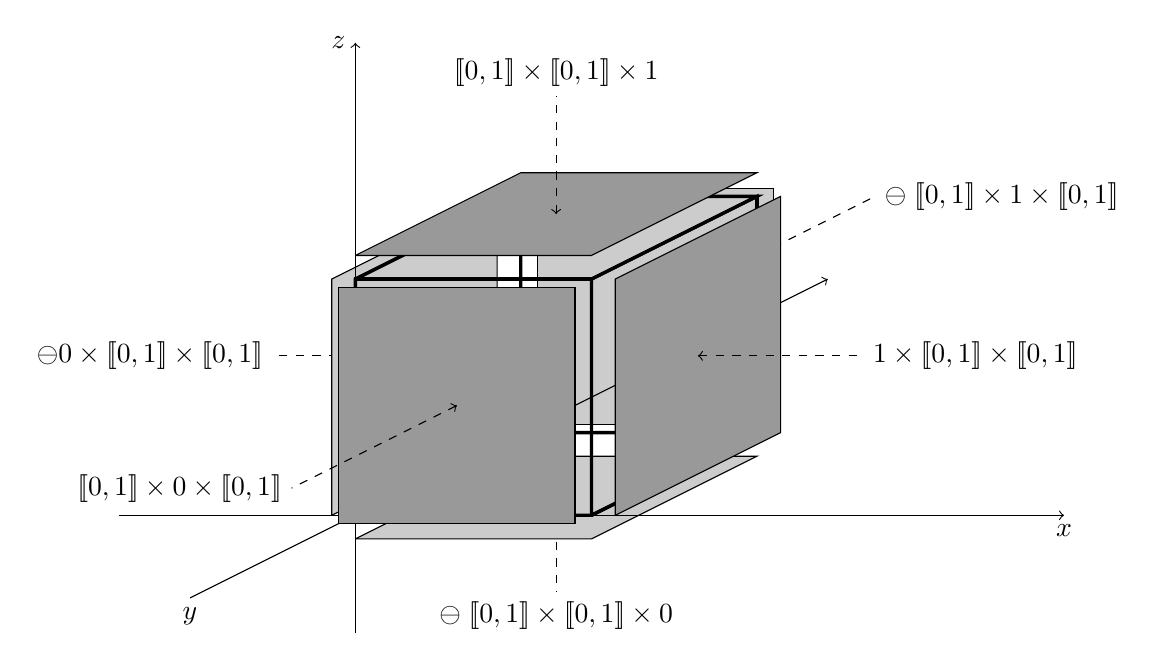
\begin{tikzpicture}[y=1.5cm, x=3cm]	
 	%axis
 	
 	%left
	\draw[color=black, dashed, <-] (0.35, 1.35) --++ (-0.7, 0) node[anchor=east, black] {$\ominus \hset{0} \times [\![0,1]\!] \times [\![0,1]\!]$};
	%back
	\draw[color=black, dashed, <-] (1.2,1.7) --++ (1,1) node[anchor=west, black] {$\ominus \; [\![0,1]\!] \times \hset{1} \times [\![0,1]\!]$};
	%bottom
	\draw[color=black, dashed, <-] (0.85,0.35) --++ (0,-1) node[anchor=north, black] {$\ominus \; [\![0,1]\!] \times [\![0,1]\!] \times \hset{0}$};
 	
 	\filldraw[fill=black!20] (0,-0.2) --++ (1,0) --++ (0.7,0.7) --++ (-1,0) --++ (-0.7,-0.7);
	\filldraw[fill=black!20] (0.77,0.77) --++ (1,0) --++ (0,2) --++ (-1,0) --++ (0, -2);
	\filldraw[fill=black!20] (-0.1,0) --++ (0,2) --++ (0.7,0.7) --++ (0,-2) --++ (-0.7,-0.7);
 	
	\draw[->] (-1,0) -- coordinate (x axis mid) (3,0) node[anchor=north] {$x$};
    	\draw[->] (0,-1) -- coordinate (y axis mid) (0,4) node[anchor=east] {$z$};
	\draw[->] (-0.7,-0.7) node[anchor=north] {$y$} --++ (2.7,2.7) ;
	
	\draw[very thick] (0,0) --++ (1,0) --++ (0.7,0.7) --++ (-1,0) --++ (-0.7,-0.7);
	\draw[very thick] (0.7,0.7) --++ (1,0) --++ (0,2) --++ (-1,0) --++ (0, -2);
	\draw[very thick] (0,0) --++ (0,2) --++ (0.7,0.7) --++ (0,-2) --++ (-0.7,-0.7);
	\draw[very thick] (0,2) --++ (1,0) --++ (0.7,0.7) --++ (-1,0) --++ (-0.7,-0.7);
	\draw[very thick] (0,0) --++ (1,0) --++ (0,2) --++ (-1,0) --++ (0, -2);
	\draw[very thick] (1,0) --++ (0,2) --++ (0.7,0.7) --++ (0,-2) --++ (-0.7,-0.7);
	
	\filldraw[fill=black!40] (0,2.2) --++ (1,0) --++ (0.7,0.7) --++ (-1,0) --++ (-0.7,-0.7);
	\filldraw[fill=black!40] (-0.07,-0.07) --++ (1,0) --++ (0,2) --++ (-1,0) --++ (0, -2);
	\filldraw[fill=black!40] (1.1,0) --++ (0,2) --++ (0.7,0.7) --++ (0,-2) --++ (-0.7,-0.7);

	%right
	\draw[color=black, dashed, <-] (1.35+0.1, 1.35) --++ (0.7, 0) node[anchor=west, black] {$\hset{1} \times [\![0,1]\!] \times [\![0,1]\!]$};
	%front
	\draw[color=black, dashed, <-] (0.5-0.07,1-0.07) --++ (-0.7,-0.7) node[anchor=east, black] {$[\![0,1]\!] \times \hset{0} \times [\![0,1]\!]$};
	%top
	\draw[color=black, dashed, <-] (0.85,2.35+0.2) --++ (0,1) node[anchor=south, black] {$[\![0,1]\!] \times [\![0,1]\!] \times \hset{1}$};
	
	
\end{tikzpicture}
\end{figure}

There are several ways to interpret and visualize the $\oplus$ and $\ominus$ sign associated with each face.
Most naturally in $\mathbb{R}^3$ for 2-rectangles is to give each a front and back side with the sign determining which to use.
Alternatively, a 2-rectangle has a boundary formed by 1-rectangles which when drawn as arrows, will all meet head-to-tail.
This induces a clockwise or counter-clockwise cycle around the edge of the rectangle and so $\circlearrowright$ and $\circlearrowleft$ are also commonly used.
This can be seen in Figure 4.4.
One may even notice that the normals produced by both are the same and choose to use that.
These are all conceptual tools, which are convenient to use particularly in $\mathbb{R}^2$ and $\mathbb{R}^3$.
There may not be such a nice physical interpretation in other spaces.


\begin{figure}[h]
\caption[Orientations of 2-rectangles]{asdfasdfasdf }
\centering
\begin{tikzpicture}

	\def\rectCycle#1#2#3#4{
		\draw[thick, ->, color=black!80] (#1,#2) -- (#3,#2);
		\draw[thick, ->, color=black!60] (#3,#2) -- (#3,#4);
		\draw[thick, ->, color=black!40] (#3, #4) -- (#1,#4);
		\draw[thick, ->, color=black!20] (#1,#4) -- (#1,#2);
		\draw[thick, ->] (#1, 0) -- (#3, 0);
		%\draw[fill] (#1,#2) circle (1 pt);
	}

	
	\rectCycle {0+1}{1} {0+2}{2};
	\draw[<->] (0,3) -- (0,0) -- (3,0);
	\draw[very thick, ->] (0,1) -- (0,2);
	\draw (0,1.5) node[anchor=east] {$+$};
	\draw (1.5,0) node[anchor=north] {$+$};
	%\draw (1.5, 1.5) node {$+$};
	\draw(1.5,1.5) node {$\;\circlearrowleft^+$};
	
	  
	\rectCycle {4+2}{1} {4+1}{2};
	\draw[<->] (4+0,3) -- (4+0,0) -- (4+3,0);
	\draw[very thick, ->] (4+0,1) -- (4+0,2);
	\draw (4+0,1.5) node[anchor=east] {$+$};
	\draw (4+1.5,0) node[anchor=north] {$-$};
	%\draw (4+1.5, 1.5) node {$-$};
	\draw(4+1.5,1.5) node {$\;\circlearrowright^-$};
	
	
	\rectCycle {8+2}{2} {8+1}{1};
	\draw[<->] (8+0,3) -- (8+0,0) -- (8+3,0);
	\draw[very thick, ->] (8+0,2) -- (8+0,1);
	\draw (8+0,1.5) node[anchor=east] {$-$};
	\draw (8+1.5,0) node[anchor=north] {$-$};
	%\draw (8+1.5, 1.5) node {$+$};
	\draw(8+1.5,1.5) node {$\;\circlearrowleft^+$};
	
	
	\rectCycle {12+1}{2} {12+2}{1};
	\draw[<->] (12+0,3) -- (12+0,0) -- (12+3,0);
	\draw[very thick, ->] (12+0,2) -- (12+0,1);
	\draw (12+0,1.5) node[anchor=east] {$-$};
	\draw (12+1.5,0) node[anchor=north] {$+$};
	%\draw (12+1.5, 1.5) node {$-$};
	\draw(12+1.5,1.5) node {$\;\circlearrowright^-$};
	
\end{tikzpicture}
\end{figure}

%%%%%%%%%%%%%%%%%%%%%%%%%%%%%%%%%%%%%%%%%
%
% CHAINS
%
%%%%%%%%%%%%%%%%%%%%%%%%%%%%%%%%%%%%%%%%%

\section{Chains}

\todo[inline]{
We have already seen chains without mentioning them explicitly.

To form the boundary, of a $k$-cube we took the sum of $(k-1)$-cubes.

These sums are commonly known as chains.}

\begin{definition}
	$C_k$ is the Abelian group generated by $k$-cubes with $\oplus$ hybrid set addition.
\end{definition}

\todo[inline]{
Since $k$-chains are linear sums of $k$-cubes.

It is natural to extend the boundary linearly to chains as well

And so $\partial_k$ becomes a map from $k$-chains to $(k-1)$-chains.

At which point it becomes natural to ask ``what does $\partial \partial$ look like?''
}

\subsection{Example: \emph{Boundary of a boundary (of a 2-cube)}}
Let $\boldsymbol{a} =(a_1,a_2)$ and $\boldsymbol{b}= (b_1,b_2)$.
We wish to compute $\partial_1 ( \partial_2 ( \; [\![\boldsymbol{a}, \boldsymbol{b} ]\!] \; ) )$

\begin{align}
	\partial_1 ( \partial_2 ( [\![ a_1 , b_1 ]\!] \times [\![a_2, b_2 ]\!] ) )
	=	& \; \ominus \partial_1( \hset{0} \times [\![0,1]\!]) \; \oplus 	\; \partial_1(\hset{1} \times [\![0,1]\!]) \notag \\
		& \; \oplus 	\partial_1( [\![0,1]\!] \times \hset{0}) \; \ominus \; \partial_1([\![0,1]\!] \times \hset{1}) \\
	=	& \ominus	( \ominus \hset{(0,0)} \oplus \hset{(0,1)} ) \; \oplus \; 	(\ominus \hset{(1,0)} \oplus \hset{(1,1)}) \notag \\
		& \oplus 	( \ominus \hset{(0,0)} \oplus \hset{(1,0)} ) \; \ominus \;	(\ominus \hset{(0,1)} \oplus \hset{(1,1)}) \\
	=	& \;\emptyset	
\end{align}

When moving from (4.16) to (4.17), in addition to applying $\partial_1$ we used the reduction, $\hset{x} \times \hset{y} = \hset{ (x,y) }$.
The identity ``$\partial \partial = 0$'' is not unique to $2$-cubes but holds for higher dimensions as well.
In fact it is one of the primary conditions for boundary operators in general.
For now we will simply prove for $n$-cubes.


\begin{figure}[h]
\caption[Boundary of a boundary (of a 2-cube)]{asdfasdfasdf }
\centering
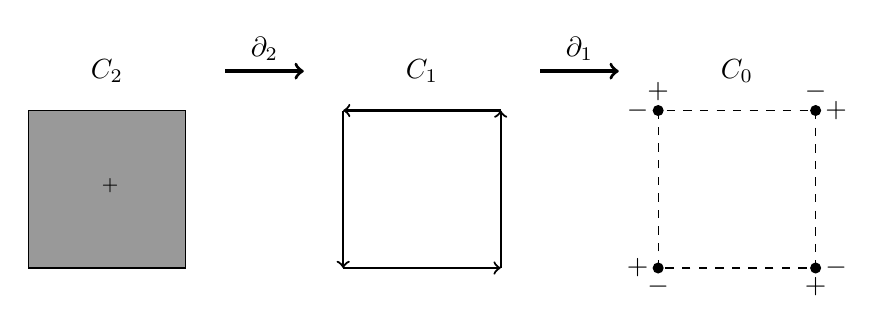
\begin{tikzpicture}

	\draw (1,2.5) node {$C_2$};
	\filldraw[fill=black!40] (0,0) rectangle (2,2);
	\draw (1,1) node {$\;\circlearrowleft^+$};
	
	\draw[very thick, ->] (2.5,2.5) --++ (0.5,0) node[anchor=south] {$\partial_2$} --++ (0.5,0);
	
	\draw (4+1,2.5) node {$C_1$};
	\draw[thick, ->] (4+0,0) --++ (2,0);
	\draw[thick, ->] (4+2,0) --++ (0,2);
	\draw[thick, ->] (4+2,2) --++ (-2,0);
	\draw[thick, ->] (4+0,2) --++ (0,-2);
	
	\draw[very thick, ->] (6.5,2.5) --++ (0.5,0) node[anchor=south] {$\partial_1$} --++ (0.5,0);
	
	\draw (8+1,2.5) node {$C_0$};
	\draw[dashed] (8+0,0) --++ (0,2) --++ (2,0) --++ (0,-2) --++ (-2,0);
	\fill (8,0) node[anchor=north] {$-$} node[anchor=east] {$+$} circle (2pt);
	\fill (8+2,0) node[anchor=west] {$-$} node[anchor=north] {$+$}  circle (2pt);
	\fill (8+2,2) node[anchor=south] {$-$} node[anchor=west] {$+$} circle (2pt);
	\fill (8,2) node[anchor=east] {$-$} node[anchor=south] {$+$} circle (2pt);
	
\end{tikzpicture}
\end{figure}

Let $[\![\boldsymbol{a}, \boldsymbol{b}]\!]$ be a $k$-rectangle in $\mathbb{R}^n$.
 
Proof of $\partial \partial = 0$



\todo[inline]{
- Chain complex
}

\begin{equation}
	\ldots \xleftarrow{\partial_{k-1}} C_{k-1} \xleftarrow{\partial_{k}} C_k \xleftarrow{\partial_{k+1}} C_{k+1} \xleftarrow{\partial_{k+2}} ...
\end{equation}

$dd=0$

But we are getting ahead of ourselves... lets look at differential forms.